\documentclass[12pt]{article}
\usepackage{amsmath, amssymb}
\usepackage{amsthm}
\usepackage{hyperref}
\usepackage{MnSymbol}
%%\usepackage[pdftex]{graphicx}
\usepackage{enumerate}
\usepackage{amsmath}
\usepackage{amssymb}
\usepackage{multicol}
\usepackage{algpseudocode}
\usepackage{algorithm}


\usepackage[final]{graphicx}
\usepackage{subcaption}
\renewcommand{\phi}{\varphi}
\newcommand{\rarrow}{\rightarrow}
\usepackage{ listings}
\title{COMP 557: Homework 2}

\author{Guangyuan Yu(gy12), Suiyi Fu(sf22)}


\begin{document}
\maketitle

\section{1}
\subsection{What is the solution}
Choose the branch on the right side.
\subsection{b.alpha-beta pruning}
10 leaves are visited. The cut off parts are in the block. Leaves with "x" are not visited. Nodes with "x" are not calculated.

\begin{figure}[H]
  \caption{center}
  \centering
    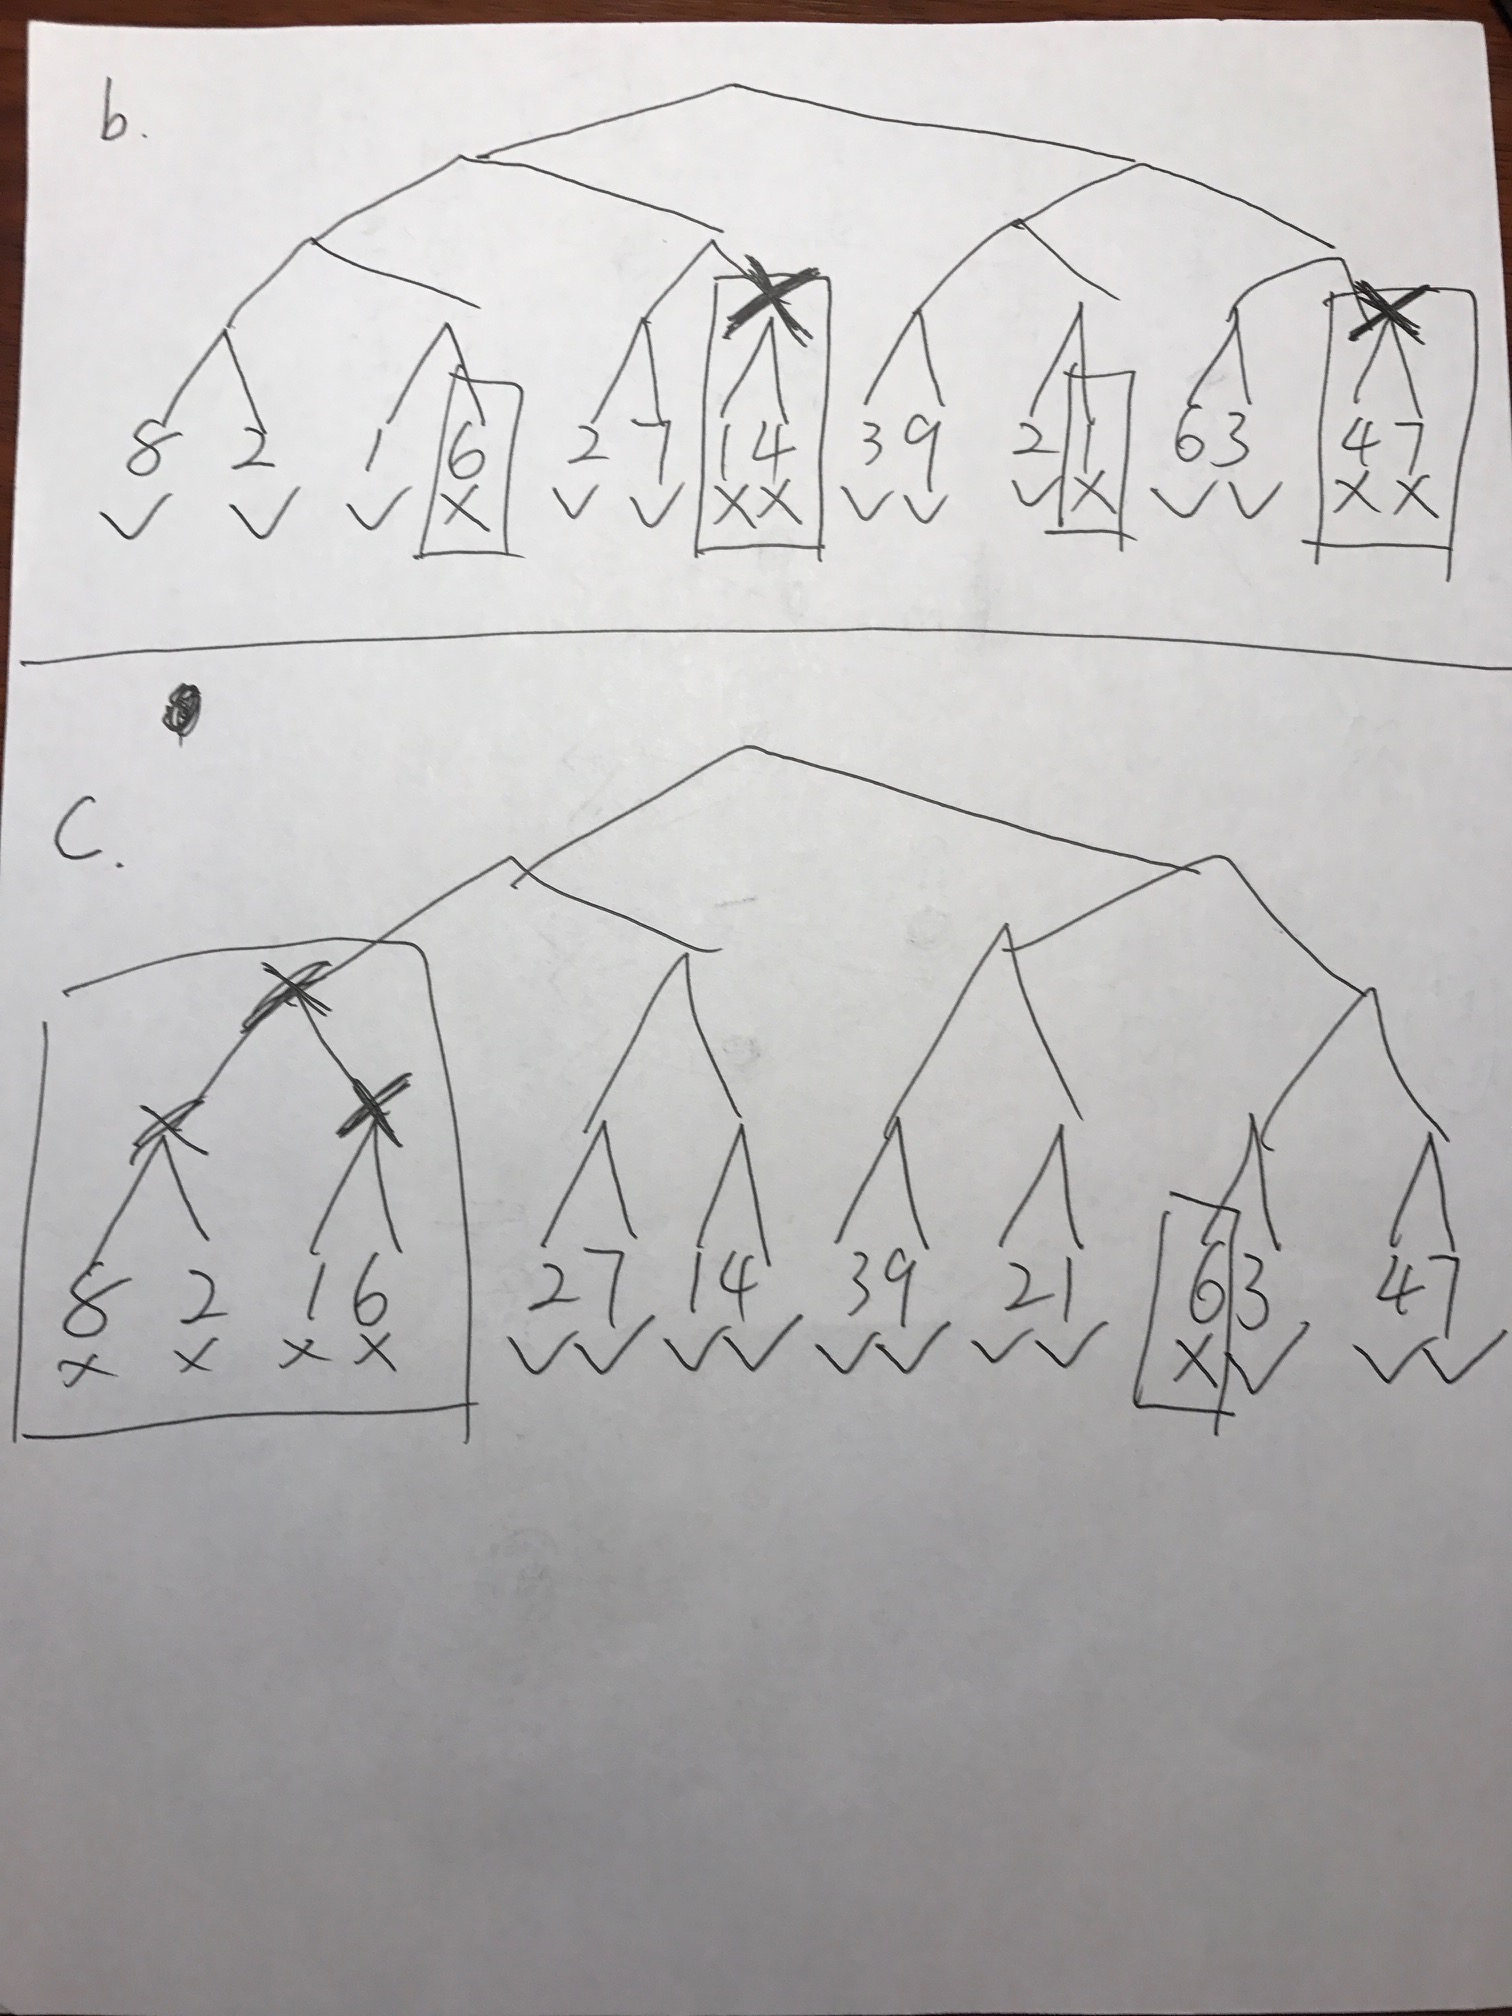
\includegraphics[scale=0.2]{3136.jpg}
\end{figure}
\subsection{c.alpha-beta pruning}
11 leaves are visited.  Leaves with "x" are not visited. Nodes with "x" are not calculated.

\subsection{d.}
If we made good choice, we can cut off more node, leading to a fast calculation. The heuristic function could be the negative difference of the two numbers on both sides. For left-to -right seach, it is 2-8=-6, for right to left search, it is 4-7=-3. We need to add a number to them to make them positive. But -6+a<-3+a is always correct, and it lead us to search from left-to-right. It is because the lowest level node is min node, the data with larger variance will contribute more to alpha and beta, which will lead to a lager cutoff.

\subsection{e.}
Because there is some goal state that takes longer time to get, or you don't know where it is, or maybe there are several goal states. So, if we start from current position, we can get the goal state which is achievable to us. 





\section{2 Minimax and expectimax}
\subsection{2.1 Draw a game tree}

			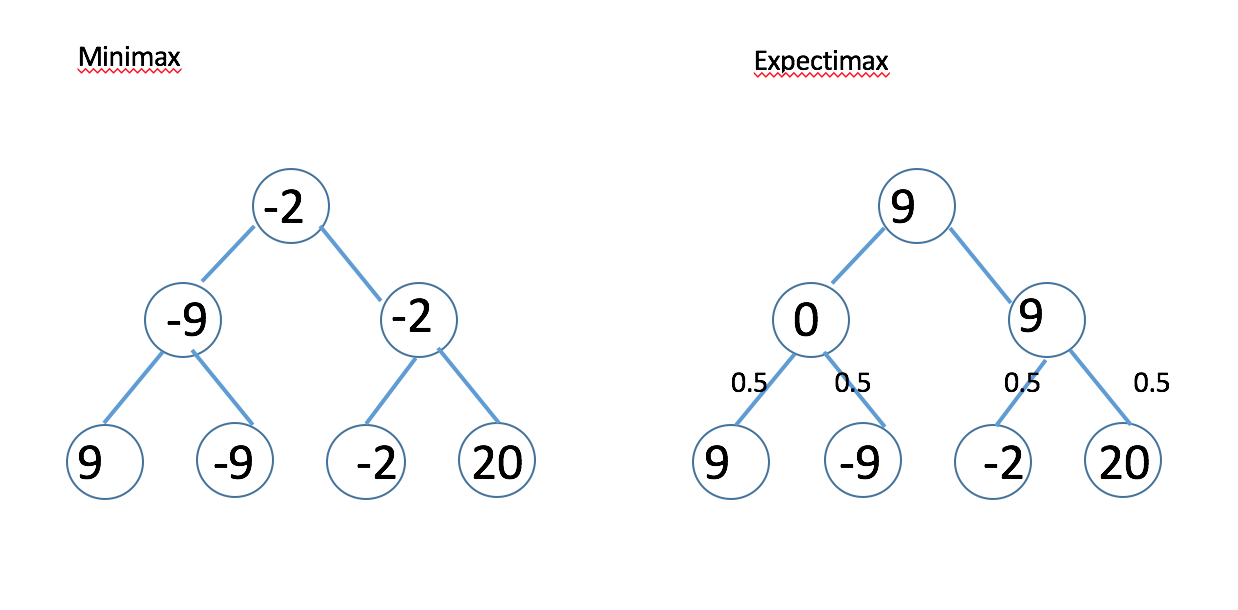
\includegraphics[scale=0.7]{p1.png}
	
	\subsection{2.2 Draw a game tree}
		\paragraph{}
			It is impossible that the value for minimax search is larger than the value of expectimax search. For minimax, the MIN player choose the worst case for the MAX player. For expectimax, since it is a chancy choice, it will improve the worst case by the average value. Thus, the adversary may choose a value that is not the worst case for the MAX player, and the value of root may increased for expectimax search. Thus, the value of minimax search could never be larger than the value of expectimax search.

	
	\subsection{2.3 assumption}
		\paragraph{}
			When player 2 is an adversarial player who plays perfectly rather than randomly, 
or if player 2 plays randomly but player 1 does not know player 2’s probability distribution, player 1 should use minimax search rather than expectimax search to select a move. 
			
	\subsection{2.4 assumtion}
		\paragraph{}
			If player1 know player2  has outcomes distribution, player1 should use expectimax search rather than minimax search. 
	
	\subsection{2.5}
		\paragraph{}
Every node has a pair of values instead of one. (rational value, mistaken value).  
Min node will make choice based on the mistaken value while max value choose nodes based on the rational value.


Take the graph in following figure as an example. 
For node E, max node will see it as 20 but min node would wrongfully calculate it as 9. Hence we have a pair of [20,9]
as value for node E. Same for other nodes D, G, H. When it comes to B, it will select path based the second value, so the pair of value [20,9] will 
be selected. Same method applies for node C. To Node A, it then select nodes based on the first value, so it will chose [20,9] And the complete path will
be: A-B-E-24 and we will have 24 as result.	
         		 \begin{center}
                        \includegraphics[scale=0.6]{p2.png}
                        \end{center}		


























\section{Multi-agent pacman}
\subsection{Warm up}
\subsection{Problem 1: Minimax}
\subsubsection{recurrence for $V_{opt}(s)$}


		\paragraph{}
		\paragraph{}
$D_{init} = d_{max} * (n+1) $

$V_{opt}(s) = V_{opt}(s, 0, D_{init})$
\[ V_{opt}(s, currentAgent, d) = 
\begin{cases} 
Utility(s)   \quad \text{if isEnd(s)}\\
Evaluation(s) \quad \text{if d = 0}  \\ \\
\substack{max \\a \in Actions(s)} V_{opt}(successor(s, currentAgent, a), nextAgent, d - 1 ) \\ \text{if it is Player[0] in Player(s)} \\ \\
\substack{min \\a \in Actions(s)} V_{opt}(successor(s,currentAgent, a), nextAgent, d - 1) \\ \text{ if it is not Player[0] in Player(s)} \\
\end{cases}
\]

\subsubsection{3.2 MinimaxAgent}

\begin{lstlisting}
python pacman.py -p MinimaxAgent -l minimaxClassic -a depth=1
value is 9
value is 8
value is 7
value is 6
value is 5
value is 4
value is -497
Pacman died! Score: -497
Average Score: -497.0
Scores:        -497
Win Rate:      0/1 (0.00)
Record:        Loss
pacman.py -p MinimaxAgent -l minimaxClassic -a depth=2
value is 8
value is 7
value is 516
value is 516
Pacman emerges victorious! Score: 516
python pacman.py -p MinimaxAgent -l minimaxClassic -a depth=3
value is 7
value is 6
value is 5
value is 4
value is -495
Pacman died! Score: -495
Average Score: -495.0
Scores:        -495
Win Rate:      0/1 (0.00)
Record:        Loss
python pacman.py -p MinimaxAgent -l minimaxClassic -a depth=4
value is -492
value is -492
Pacman died! Score: -492
Average Score: -492.0
Scores:        -492
Win Rate:      0/1 (0.00)
Record:        Loss



\end{lstlisting}
I run it for 20 times
\begin{lstlisting}
python pacman.py -p MinimaxAgent -l minimaxClassic -a depth=4 -n 20
Pacman emerges victorious! Score: 516
Pacman emerges victorious! Score: 516
Pacman emerges victorious! Score: 516
Pacman emerges victorious! Score: 516
Pacman emerges victorious! Score: 516
Pacman emerges victorious! Score: 516
Pacman died! Score: -495
Pacman emerges victorious! Score: 516
Pacman emerges victorious! Score: 516
Pacman emerges victorious! Score: 516
Pacman emerges victorious! Score: 516
Pacman emerges victorious! Score: 516
Pacman died! Score: -494
Pacman emerges victorious! Score: 516
Pacman emerges victorious! Score: 516
Pacman emerges victorious! Score: 516
Pacman emerges victorious! Score: 516
Pacman emerges victorious! Score: 516
Pacman emerges victorious! Score: 516
Pacman emerges victorious! Score: 516
Average Score: 414.95
Scores:        516, 516, 516, 516, 516, 516, -495, 516, 516, 516, 516, 516, -494, 516, 516, 516, 516, 516, 516, 516
Win Rate:      18/20 (0.90)
Record:        Win, Win, Win, Win, Win, Win, Loss, Win, Win, Win, Win, Win, Loss, Win, Win, Win, Win, Win, Win, Win
\end{lstlisting}



\subsubsection{Why does pacman thrash around right next to a dot? Place your explanation in writeup.pdf. }



No matter when the pacman eat the dot, the score will increase. The pacman doesn't worry about the time. Therefore, he would thrash around to a dot. 


\subsubsection{Why does pacman rush to the closest ghost in minimax search on trappedClassic? Place your explanation in writeup.pdf.}

The trapped Classic layout is designed in such a way that pacman could not find a path to eat food before being killed. Since pacman can not get any points by eating food while his being alive will only take points off, so pacman go to the ghost to decrease the points that will be taken off every time frame.











\subsection{Problem 2: Alpha-beta pruning }
\begin{lstlisting}
python pacman.py -p AlphaBetaAgent -l minimaxClassic -a depth=3
value is  7
value is  6
value is  5
value is  -495
value is  -495
Pacman died! Score: -495
Average Score: -495.0
Scores:        -495
Win Rate:      0/1 (0.00)
Record:        Loss
python pacman.py -p AlphaBetaAgent -l minimaxClassic -a depth=4
value is  -492
value is  5
value is  516
value is  516
Pacman emerges victorious! Score: 516
Average Score: 516.0
Scores:        516
Win Rate:      1/1 (1.00)
Record:        Win


python pacman.py -p AlphaBetaAgent -l minimaxClassic -a depth=2
value is  8
value is  7
value is  516
value is  516
Pacman emerges victorious! Score: 516
Average Score: 516.0
Scores:        516
Win Rate:      1/1 (1.00)
Record:        Win

python pacman.py -p AlphaBetaAgent -l minimaxClassic -a depth=1
value is  9
value is  8
value is  7
value is  516
Pacman emerges victorious! Score: 516
Average Score: 516.0
Scores:        516
Win Rate:      1/1 (1.00)
Record:        Win


\end{lstlisting}
Right now the win rate for miniClassic layout is 
\begin{lstlisting}
Win Rate:      11/20 (0.55)
Record:        Win, Win, Loss, Loss, Win, Loss, Loss, Loss, Win, Win, Win, Loss, Win, Win, Win, Win, Win, Loss, Loss, Loss
\end{lstlisting}






\subsection{3.4 Problem 3: Expectimax  }
\subsubsection{Recurrence of $V_{opt}$}
\paragraph{}
\paragraph{}

$D_{init} = d_{max} * (n+1) $
\paragraph{}
$V_{opt}(s) = V_{opt}(s, D_{init}, 0)$


\[ V_{opt}(s, d, currentAgent) = 
\begin{cases} 
Utility(s)   \quad \text{if isEnd(s)}\\
Evaluation(s) \quad \text{if d = 0}  \\ \\
\substack{max \\a \in Actions(s)} V_{opt}(successor(s, currentAgent, a), d - 1, nextAgent) \\ \text{if it is Player[0] in Player(s)} \\ \\
\\
\ \dfrac{\substack{sum \\a \in Actions(s)} V_{opt}(successor(s,currentAgent, a), d - 1, nextAgent)}{length of [Actions(s)]} \\ \text{ if it is not Player[0] in Player(s)} \\
\end{cases}
\]


Right now the win rate is:
\begin{lstlisting}	
python pacman.py -p ExpectimaxAgent -l trappedClassic -a depth=3 -n 20
Win Rate:      10/20 (0.50)
Record:        Win, Loss, Win, Loss, Win, Win, Loss, Loss, Loss, Loss, Loss, Win, Loss, Loss, Win, Loss, Win, Win, Win, Win


\end{lstlisting}






\subsubsection{Why does pacman  behavior in expectimax differ from the minimax case (i.e., why doesnot he head directly for the ghosts)? Place your answer in writeup.pdf.}
When the ghost takes the worst behavior, it is minimax game, but the ghost don't always take the worst action, so the pacman can get some advantage. Once the pacman knows the distribution of ghost, the pacman can be more aggressive, while the minimax search always try to avoid the worst situation. 
In expectimax search, the pacman know the ghost would not always take the worst action against him, so he can take some risk and get more food. So he doesn't need die as quickly as before.



\subsection{Problem 4: Evaluation function}




Right now, we want to use two kinds of award in evaluation, food and ghost. When the food are less left, and eating food right now will give pacman higher score. As for the ghost, the distance is large from pacman will bring a higher score.

We also take into the lifetime into consideration, if the future step will lead to death, the score will be very low. 

\begin{lstlisting}
python pacman.py -l smallClassic -p ExpectimaxAgent -a evalFn=better -q -n 10

Average Score: 829.7
Scores:        1059, -349, 943, 905, 935, 1112, 955, 1263, 901, 573
Win Rate:      9/10 (0.90)
Record:        Win, Loss, Win, Win, Win, Win, Win, Win, Win, Win
\end{lstlisting}





\section{Expectimax search and pruning}
	\subsection{}
		\paragraph{}

No, it is impossible. Since the leaf values are unbounded, the next branch of the tree may include larger values than the branches before. That is to say, the next branch can not be cut off. We have to examine all nodes to find the best leaf value and assign it to the root node eventually.


	
	\subsection{}
		\paragraph{}
No, it is impossible. The next branch of the tree may include larger values than the branches before at the max node.  The leaf value is unbounded and chance nodes have non-zero probabilities for all outcomes, which will make the value of chance nodes unbounded. So we have to examine all nodes to find the best.
		

	
	\subsection{}
		\paragraph{}

 It is possible. See figure here. A B C are all max node. If the value of B is 1. You don?t need to check node C because the value of C (max value) cannot larger than 1.
		\paragraph{}
			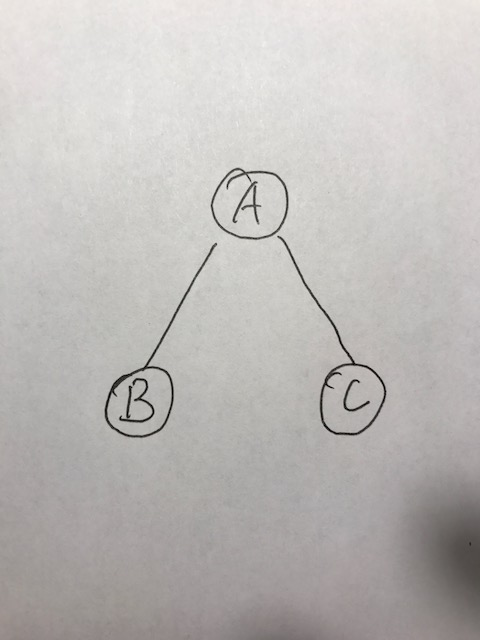
\includegraphics[scale=0.2]{3137.jpg}
			
	
	\subsection{}
		\paragraph{}
It is possible. See the same picture. A is the max node. B C are chance nodes. If the value of B is 1. You don?t need to check node C because the value on C (expectation value) cannot larger than 1.

		
	
	\subsection{}
		\paragraph{}
If the value of the leaf nodes are not bounded, it doesn't make a difference. If the value of the leaf nodes are bounded, searching highest probability first can be more helpful to lower the upper bound of chance node value that can be more helpful to generate the opportunities of pruning. 
		

\end{document}

